%
% Author: David Oniani
%
%  _____    ___     _  __
% |_   _| _|_ _|___| |/ /___
%   | || '__| |/ __| ' // __|
%   | || |  | | (__| . \\__ \
%   |_||_| |___\___|_|\_\___/
%

%%%%%%%%%%%%%%%%%%%%%%%%%%%%%%%%%%%%%%%%%%%%%%%%%%%%%%%%%%%%%%%%%%%%%%%%%%%%%%%
% Document Definition
%%%%%%%%%%%%%%%%%%%%%%%%%%%%%%%%%%%%%%%%%%%%%%%%%%%%%%%%%%%%%%%%%%%%%%%%%%%%%%%

\documentclass[11pt]{article}

%%%%%%%%%%%%%%%%%%%%%%%%%%%%%%%%%%%%%%%%%%%%%%%%%%%%%%%%%%%%%%%%%%%%%%%%%%%%%%%
% Packages and Related Settings
%%%%%%%%%%%%%%%%%%%%%%%%%%%%%%%%%%%%%%%%%%%%%%%%%%%%%%%%%%%%%%%%%%%%%%%%%%%%%%%

% Global, document-wide settings
\usepackage[margin=1in]{geometry}
\usepackage[utf8]{inputenc}
\usepackage[english]{babel}

% Other essential packages
\usepackage{booktabs}
\usepackage{hyperref}
\usepackage{minted}
\usepackage{tocloft}
\usepackage{xcolor}

% Packages for making a fancy-looking cover
\usepackage{afterpage}
\usepackage{tikz}
\usetikzlibrary{fadings}

%%%%%%%%%%%%%%%%%%%%%%%%%%%%%%%%%%%%%%%%%%%%%%%%%%%%%%%%%%%%%%%%%%%%%%%%%%%%%%%
% Setup
%%%%%%%%%%%%%%%%%%%%%%%%%%%%%%%%%%%%%%%%%%%%%%%%%%%%%%%%%%%%%%%%%%%%%%%%%%%%%%%

% Remove indentations from paragraphs
\setlength{\parindent}{0pt}

% PDF information and nice-looking urls
\hypersetup{%
    pdfauthor={David Oniani},
    pdftitle={Tricks},
    pdfsubject={Algorithms, Data Structures, Tricks},
    pdfkeywords={Algorithms, Data Structures, Tricks},
    pdflang={English},
    colorlinks=true,
    linkcolor={black!50!blue},
    citecolor={black!50!blue},
    urlcolor={black!50!blue}
}

% Font size for minted
\setminted{fontsize=\footnotesize}

% Colorscheme for minted
\usemintedstyle{tango}

% Dots for ToC
\renewcommand{\cftsecleader}{\cftdotfill{\cftdotsep}}

% Fancy cover
\newgeometry{left=1in,right=1in,top=1in,bottom=0in}

\DeclareFixedFont{\titlefont}{T1}{ppl}{n}{}{0.8in}
\DeclareFixedFont{\subtitlefont}{T1}{ppl}{n}{}{0.4in}

\definecolor{color}{HTML}{3c2ac7}
\pagecolor{color}

\afterpage{\restoregeometry}
\afterpage{\nopagecolor}

%%%%%%%%%%%%%%%%%%%%%%%%%%%%%%%%%%%%%%%%%%%%%%%%%%%%%%%%%%%%%%%%%%%%%%%%%%%%%%%
% Author(s), Title, and Date
%%%%%%%%%%%%%%%%%%%%%%%%%%%%%%%%%%%%%%%%%%%%%%%%%%%%%%%%%%%%%%%%%%%%%%%%%%%%%%%

% Author(s)
% \author{David Oniani\\
%     \href{mailto:onianidavid@gmail.com}{onianidavid@gmail.com}}

% Title
% \title{\textbf{Tricks}\\
%     {\small\textsuperscript{*}Various Algorithmic Tricks for a Great Good!}}

% Date
% \date{\today}

%%%%%%%%%%%%%%%%%%%%%%%%%%%%%%%%%%%%%%%%%%%%%%%%%%%%%%%%%%%%%%%%%%%%%%%%%%%%%%%
% Beginning of the Document
%%%%%%%%%%%%%%%%%%%%%%%%%%%%%%%%%%%%%%%%%%%%%%%%%%%%%%%%%%%%%%%%%%%%%%%%%%%%%%%

\begin{document}
% \maketitle

\begin{flushleft}
    \rule{\paperwidth - 150pt}{1pt}
    \\
    \vspace{0.5em}
    \titlefont tricks
    \\
    \vspace{0.25em}
    \subtitlefont by David Oniani
    \\
    \rule{\paperwidth - 150pt}{1pt}
\end{flushleft}
\vfill
\begin{tikzpicture}
    \centering
    \node[scope fading=north,inner sep=0pt,outer sep=0pt] {
        \makebox[\linewidth]{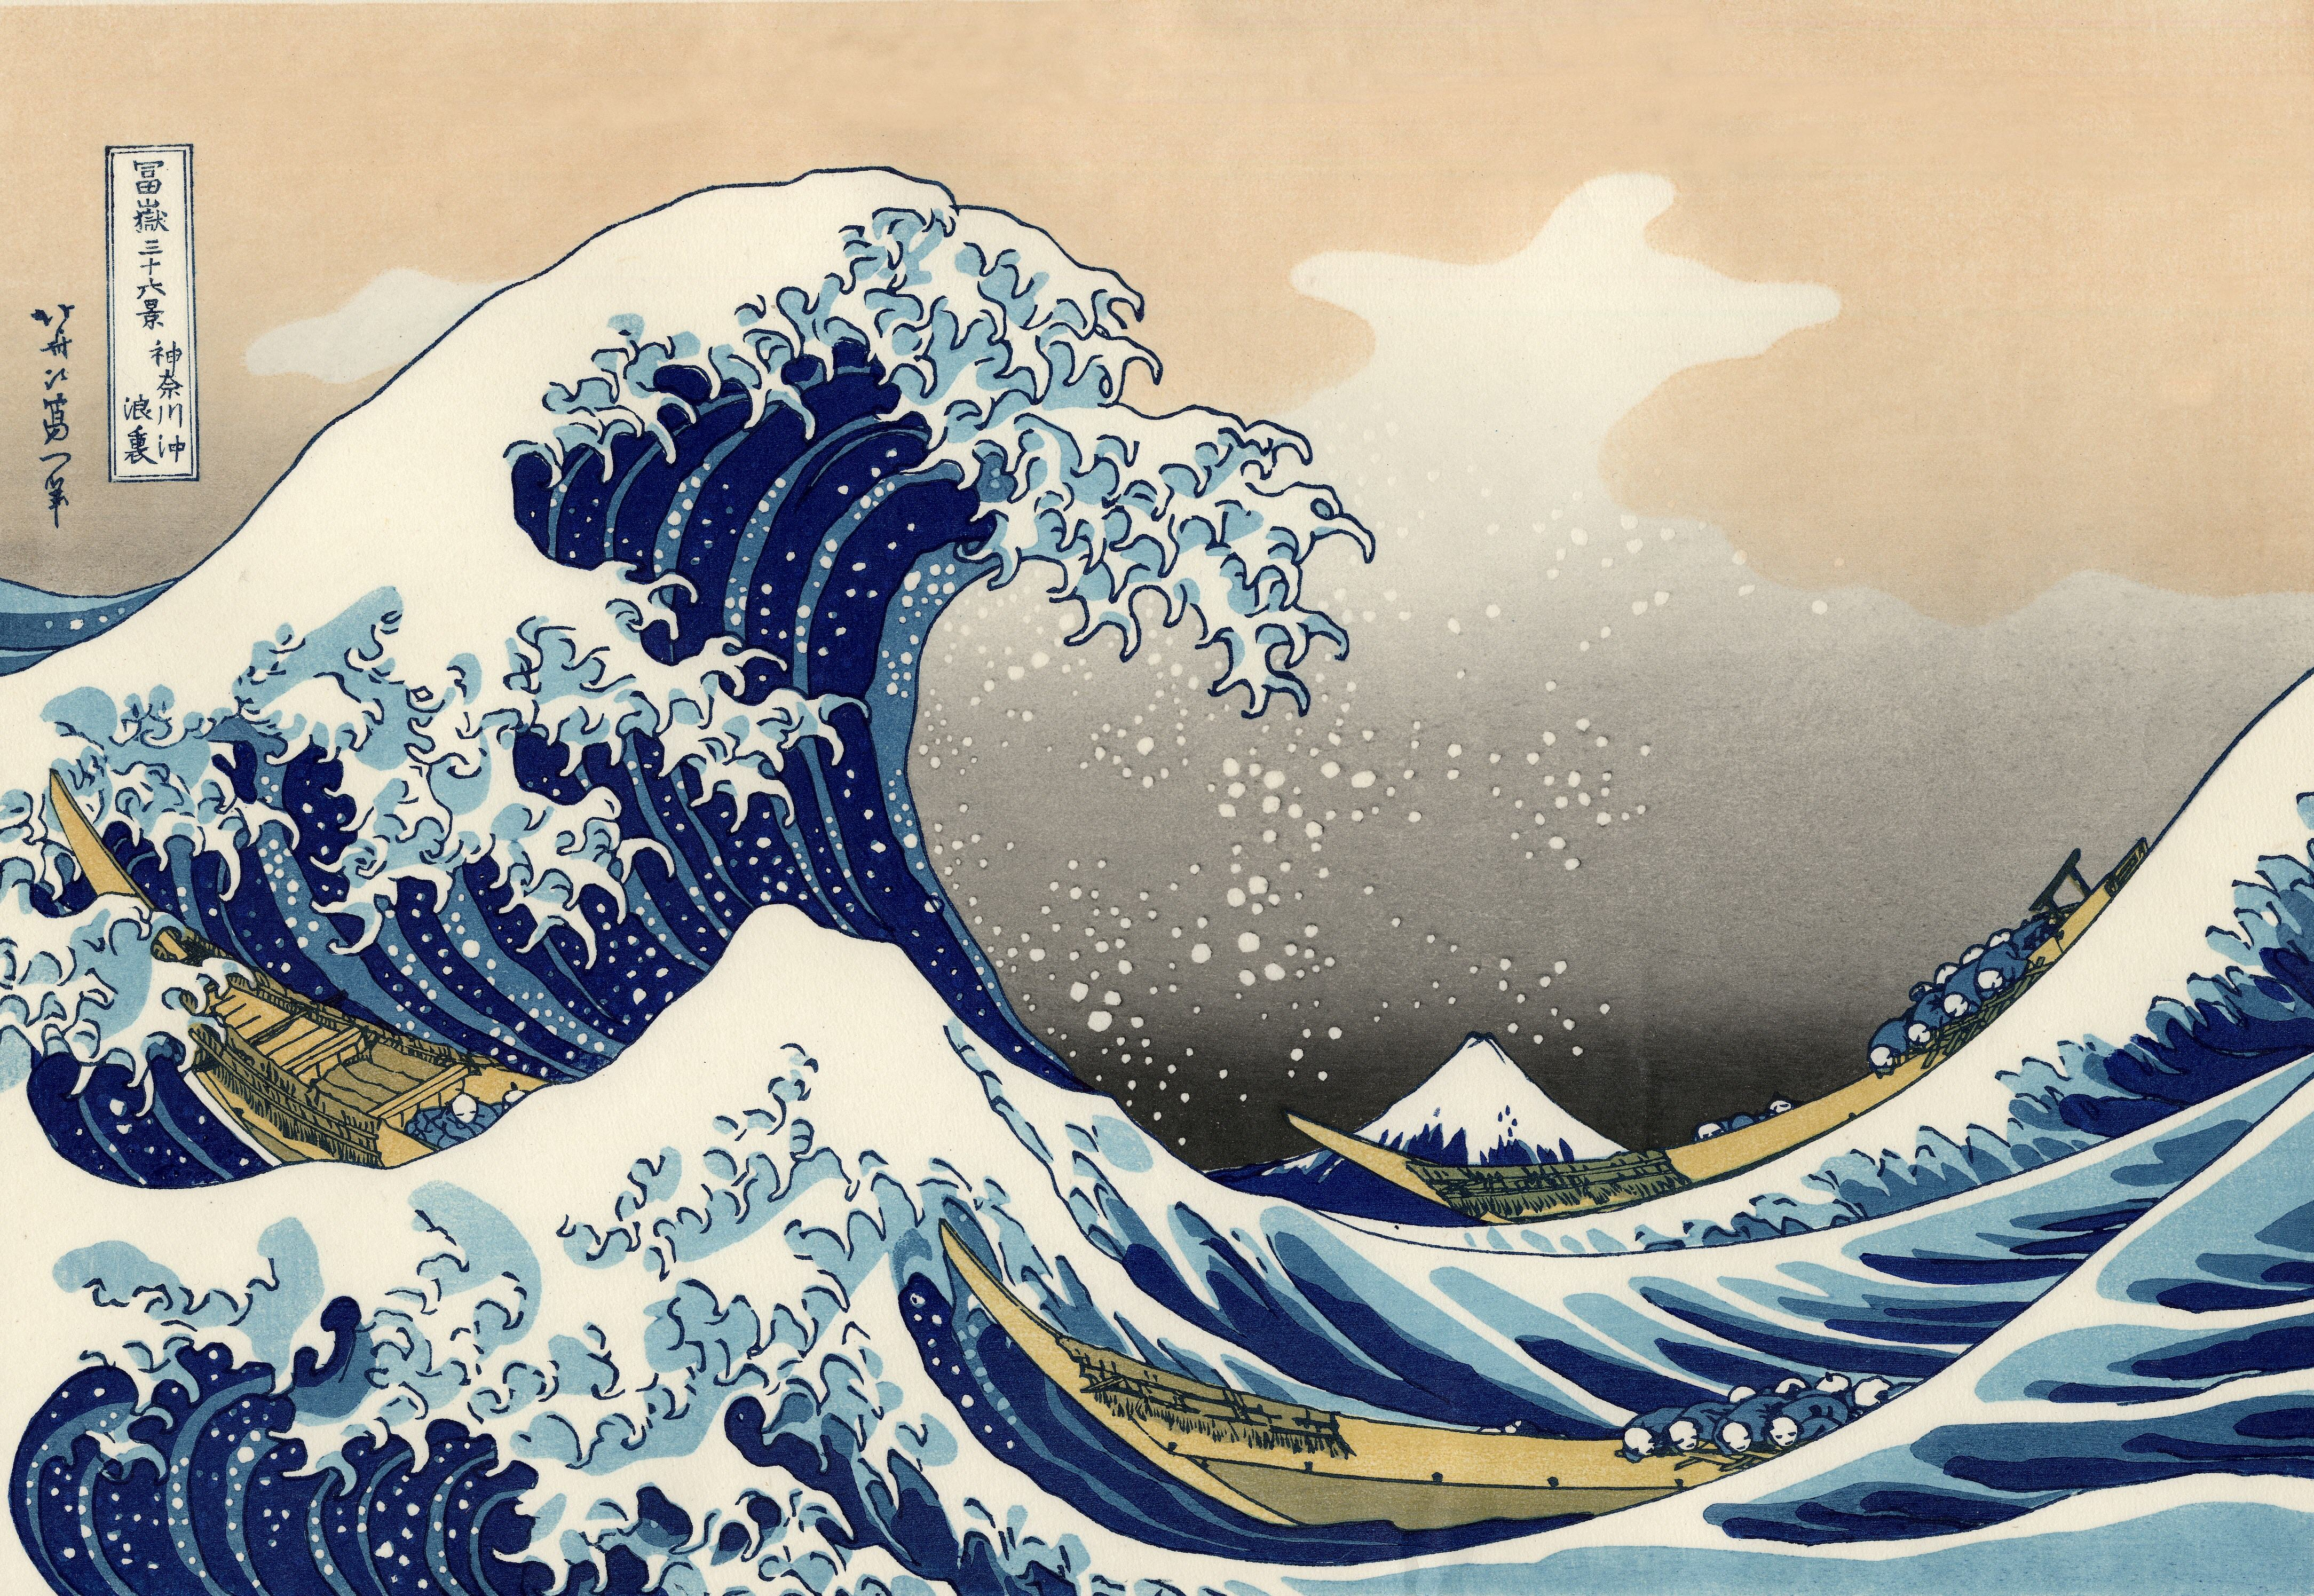
\includegraphics[width=\paperwidth]{cover.jpg}}
    };
\end{tikzpicture}

%%%%%%%%%%%%%%%%%%%%%%%%%%%%%%%%%%%%%%%%%%%%%%%%%%%%%%%%%%%%%%%%%%%%%%%%%%%%%%%
% Table of Contents
%%%%%%%%%%%%%%%%%%%%%%%%%%%%%%%%%%%%%%%%%%%%%%%%%%%%%%%%%%%%%%%%%%%%%%%%%%%%%%%

\clearpage
\tableofcontents
\clearpage

%%%%%%%%%%%%%%%%%%%%%%%%%%%%%%%%%%%%%%%%%%%%%%%%%%%%%%%%%%%%%%%%%%%%%%%%%%%%%%%
% Trie - A Prefix Tree
%%%%%%%%%%%%%%%%%%%%%%%%%%%%%%%%%%%%%%%%%%%%%%%%%%%%%%%%%%%%%%%%%%%%%%%%%%%%%%%

\section{Trie - A Prefix Tree}

There are many ways to constuct a trie. We will use a hash map based approach.
We first create a \mintinline{python}{Node} class.

\begin{figure}[H]
    \centering
    \begin{minted}{python}
        class TrieNode:
            def __init__(self) -> None:
                """Initialize the `TrieNode` class."""

                self._children: dict[str, TrieNode] = {}
                self._isendofword: bool = False
    \end{minted}
\end{figure}

We can now design the trie data structure. The initializer will only contain a
root of the trie.

\begin{figure}[H]
    \centering
    \begin{minted}{python}
        class Trie:
            def __init__(self) -> None:
                """Initialize the `Trie` class."""

                self._root = TrieNode()
    \end{minted}
\end{figure}

Now, the first method to implement is the insertion operation. If we cannot
insert a word into a trie, we are not going to be able to do much with it. The
algorithm is very straightforward. One iterates over all characters in the word
to be inserted and checks if the characters is in the children of the current
node. If it is, follow the path of that node. If not, create a new node at that
position and once again, follow that road.

\begin{figure}[H]
    \centering
    \begin{minted}{python}
        def insert(self, word: str) -> None:
            """Initialize the `Trie` class."""

            ptr: Node = self._root
            for char in word:
                if char not in ptr._children:
                    ptr._children[char] = TrieNode()
                ptr = ptr._children[char]

            ptr._isendofword = True
    \end{minted}
\end{figure}

One of the primary features of the trie is to be able to search for a word.
The implementation of this algorithm is shown below.

\begin{figure}[H]
    \centering
    \begin{minted}{python}
        def search(self, word: str) -> bool:
            """Check if a trie contains a given word."""

            ptr: Node = self._root
            for char in word:
                if char not in ptr._children:
                    return False
                ptr = ptr._children[char]

            return ptr._isendofword
    \end{minted}
\end{figure}

Similarly, searching a prefix is also very important. It looks almost exactly
the same as the code for searching a word.

\begin{figure}[H]
    \centering
    \begin{minted}{python}
        def prefix_search(self, word: str) -> bool:
            """Check if a trie contains a given prefix."""

            ptr: Node = self._root
            for char in word:
                if char not in ptr._children:
                    return False
                ptr = ptr._children[char]

            return True
    \end{minted}
\end{figure}

%%%%%%%%%%%%%%%%%%%%%%%%%%%%%%%%%%%%%%%%%%%%%%%%%%%%%%%%%%%%%%%%%%%%%%%%%%%%%%%
% Merge Sort
%%%%%%%%%%%%%%%%%%%%%%%%%%%%%%%%%%%%%%%%%%%%%%%%%%%%%%%%%%%%%%%%%%%%%%%%%%%%%%%

\newpage

\section{Merge Sort}

Merge sort is one of the simplest sorting algorithms that scales very well. It
relies on two operations - \mintinline{python}{merge} and
\mintinline{python}{sort}.

\begin{figure}[H]
    \centering
    \begin{minted}{python}
        def merge(arr1: list[int], arr2: list[int]) -> list[int]:
            """Merge two sorted lists."""

            res: list[int] = []

            i: int = 0
            j: int = 0
            while i <= len(arr1) - 1 and j <= len(arr2) - 1:
                if arr1[i] <= arr2[j]:
                    res.append(arr1[i])
                    i += 1
                else:
                    res.append(arr2[j])
                    j += 1
            
            while i <= len(arr1) - 1:
                res.append(arr1[i])
                i += 1

            while j <= len(arr2) - 1:
                res.append(arr2[j])
                j += 1

            return res
    \end{minted}
\end{figure}

We now need to implement the sort function.


\begin{figure}[H]
    \centering
    \begin{minted}{python}
        def sort(arr: list[int]) -> list[int]:
            """Performs a merge sort."""

            if len(nums) <= 1:
                return nums
            
            mid: int = len(arr) // 2
            left: list[int] = sort(arr[:mid])
            right: list[int] = sort(arr[mid:])

            return merge(left, right)
    \end{minted}
\end{figure}

%%%%%%%%%%%%%%%%%%%%%%%%%%%%%%%%%%%%%%%%%%%%%%%%%%%%%%%%%%%%%%%%%%%%%%%%%%%%%%%
% Levenshtein Distance
%%%%%%%%%%%%%%%%%%%%%%%%%%%%%%%%%%%%%%%%%%%%%%%%%%%%%%%%%%%%%%%%%%%%%%%%%%%%%%%

\newpage

\section{Levenshtein Distance (Edit Distance)}

Given two strings \mintinline{python}{word1} and \mintinline{python}{word2}, we
need to find the optimal/minimum number of operations required to convert
\mintinline{python}{word1} to \mintinline{python}{word2}. We are permitted the
following four operations:

\begin{enumerate}
    \item Insert a character
    \item Delete a character
    \item Replace a character
    \item Keep a character
\end{enumerate}

We take the bottom-up dynamic programming approach:

\begin{figure}[H]
    \centering
    \begin{minted}{python}
        def levenshtein_distance(word1: str, word2: str) -> int:
            """Computes the Levenshtein's distance between two words."""

            # Get the lengths
            m: int = len(word1)
            n: int = len(word2)

            # Prepopulate the DP matrix
            dp: list[list[int]] = [
                [0 for _ in range(n + 1)] for _ in range(m + 1)
            ]

            # Initialize the DP matrix with base cases
            for i in range(1, m + 1):
                dp[i][0] += i
            for j in range(1, n + 1):
                dp[0][j] += j

            # Fill the DP Matrix
            for i in range(1, m + 1):
                for j in range(1, n + 1):
                    left: int = dp[i][j - 1]
                    top: int = dp[i - 1][j]
                    top_left: int = dp[i - 1][j - 1]

                    # If characters are equal, just copy the diagonal value
                    if word1[i - 1] == word2[j - 1]:
                        dp[i][j] = top_left
                    # Otherwise, take the minimum of three adjacent cells and
                    # increment the result by one
                    else:
                        dp[i][j] = min(left, top, top_left) + 1

            # Return the optimal solution
            return dp[m][n]
    \end{minted}
\end{figure}

%%%%%%%%%%%%%%%%%%%%%%%%%%%%%%%%%%%%%%%%%%%%%%%%%%%%%%%%%%%%%%%%%%%%%%%%%%%%%%%
% Balanced Parentheses
%%%%%%%%%%%%%%%%%%%%%%%%%%%%%%%%%%%%%%%%%%%%%%%%%%%%%%%%%%%%%%%%%%%%%%%%%%%%%%%

\newpage

\section{Balanced Parentheses}

The parentheses in a string are balanced if and only if the following two
conditions are met:

\begin{enumerate}
    \item The number of \mintinline{python}{"("} and \mintinline{python}{")"}
          are equal
    \item Scanning through the string from left to right and counting how many
          \mintinline{python}{"("} and \mintinline{python}{")"} there are so
          far, there should never be a time where there are more
          \mintinline{python}{")"} than \mintinline{python}{"("}. We denote the
          balance of the string as
          \mintinline{python}{balance = count("(") - count(")")}
\end{enumerate}

If we only allow for \mintinline{python}{"()"} pair of parentheses, then the
following will check if the parenthesis are balanced:

\begin{figure}[H]
    \centering
    \begin{minted}{python}
        def is_balanced(string: str) -> bool:
            """Check if a given string has balanced parentheses."""

            balance: int = 0
            for char in string:
                if char == "(":
                    balance += 1
                elif char == ")":
                    balance -= 1

                if balance < 0:
                    return False

            return balance == 0
    \end{minted}
\end{figure}

If we allow for more than one pair of parentheses, the following stack-based
implementation generalizes well:

\begin{figure}[H]
    \centering
    \begin{minted}{python}
        def is_balanced(string: str) -> bool:
            """Check if a given string has balanced parentheses."""

            stack: list[str] = []
            closing: dict[str, str] = {")": "(", "}": "{", "]": "["}
            opening: set[str] = set(closing.values())
            for char in string:
                if char in opening:
                    stack.append(char)
                elif char in closing:
                    if not stack or closing[char] != stack.pop():
                        return False

            return not stack
    \end{minted}
\end{figure}

%%%%%%%%%%%%%%%%%%%%%%%%%%%%%%%%%%%%%%%%%%%%%%%%%%%%%%%%%%%%%%%%%%%%%%%%%%%%%%%
% The End of the Document
%%%%%%%%%%%%%%%%%%%%%%%%%%%%%%%%%%%%%%%%%%%%%%%%%%%%%%%%%%%%%%%%%%%%%%%%%%%%%%%

\end{document}
